\documentclass[12pt, times new roman, a4paper]{article}
\linespread{1,5}
\usepackage[utf8]{inputenc}
\usepackage{graphicx}
\renewcommand{\figurename}{Gambar}

\title{Oracle Application Express}
\author{Ariq Rafi Kusumah (1184076)}
\date{October 2019}
\begin{document}
\maketitle
\section{Apa itu Oracle Apex}

Platform pengembangan kode rendah yang memungkinkan anda membangun
aplikasi perusahaan yang dapat diskalakan dan aman dengan fitur world-class yang dapat digunakan perangkat lunak apapun.\\

\begin{figure}[h]
	\centering
		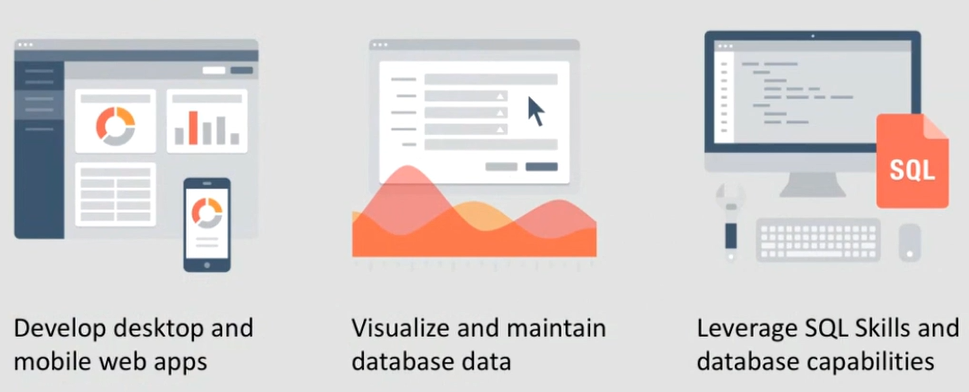
\includegraphics[scale=0.5]{Gambar/2}
	\caption{Gambar Oracle APEX}
\end{figure}

\section{Oracle APEX: Pengembangan Aplikasi Pertama Data Rendah}

\begin{figure}[h]
	\centering
		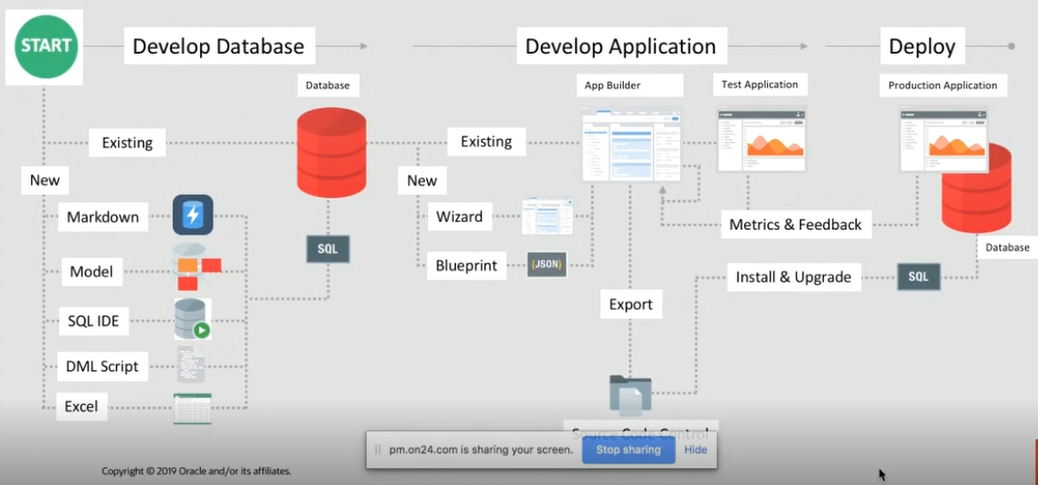
\includegraphics[scale=0.5]{Gambar/1}
	\caption{Pengembangan Aplikasi Pertama Data Rendah}
\end{figure}

\section{Mengelola Data dalam Spreadsheet Menantang}

1. Validasi Data - manual dan rawan kesalahan\\
2. Integritas Data - tidak dapat menjamin keakuratan data dalam 	 lingkungan multi-pengguna\\
3. keamanan data - penguncian sel tidak efektif\\
4. Berbagi data - Excel lamban dan sulit untuk dibagikan\\

\section{Jenis Aplikasi Yang Cocok Untuk Apex Oracle}

1. Large mission-critical apps for thousand of users\\
2. Fill in gaps in corporate systems\\
3. Steamline outed business processes\\
4. Modernization of legacy systems\\
5. Self-service apps for all employees\\
6. Customer/Partner-facing portals\\
7. proof of concepts\\
8. Quick =-win apps (lifespan < a few months\\
9. Replacing spreadsheets\\

\section{Oracle APEX: Use Cases}

\textbf{1.) Memodernisasi Formulir Oracle}\\
\textbf{Fitur}\\
1. Seret dan Jatuhkan file xls, CSV, XML, atau JSON\\
2. Buat tabel dalam Database Autonomous\\
3. Unggah Aplikasi berdasarkan tabel baru\\
\textbf{Solusi}\\
1. sumber kebenaran tunggal\\
2. Kirim URL bukan file\\
3. Aplikasi yang aman, terukur, multi-pengguna\\
4. Perluas dengan Bagan, Kalender, Validasi, dan banyak lagi\\
\textbf{2.) Pengembangan Aplikasi yang Cepat}\\
\textbf{Fitur}\\
1. Membangun aplikasi dalam beberapa hari / minggu bukan bulan / tahun\\
2. Gunakan penyihir yang kuat untuk membuat aplikasi berfitur lengkap\\
3. Mudah dimodifikasi untuk memenuhi perubahan persyaratan\\
4. Dengan cepat beralih ke aplikasi yang siap produksi\\
5. Kemampuan kode rendah memungkinkan profesional non-IT juga membangun atau membantu membangun aplikasi\\
\textbf{Solusi}\\
1. Oportunistik\\
2. Aplikasi taktis sederhana untuk memenuhi kebutuhan mendesak\\
3. Webify proses kertas\\
4. Umumnya dikembangkan oleh satu atau dua orang\\
\textbf{3.) Memperluas Sistem Perusahaan}\\
\textbf{Fitur}\\
1. Perluas ERP dan perangkat lunak perusahaan lainnya\\
2. Menyediakan dasbor khusus organisasi\\
3. Alur kerja yang ditingkatkan\\
4. Isi celah\\
\textbf{Solusi}\\
1. Memenuhi persyaratan non-standar\\
2. Optimalkan fungsi bisnis umum\\
3. Tingkatkan pengambilan data\\
4. Mengintegrasikan sumber data yang berbeda\\

\section{Oracle APEX: Distinguishing Characteristics}
Development IDE adalah browser web. Tidak diperlukan perangkat lunak klien,aplikasi disimpan dalam database sebagai data meta. Deklaratif- Tidak ada pembuatan kode,halaman efisien dengan hanya satu request dan satu respons. Pemrosesan data dilakukan dalam Database\\

\section{Fitur Tanpa Biaya dari Database Oracle}
\textbf{Fitur yang didukung penuh tanpa biaya} \\
1. Sejumlah aplikasi, Pengembang dan pengguna akhir\\
2. Tim Dukungan Oracle Khusus\\
3. 11gR2, 12c, 18c\\
4. Semua edisi DB: EE, SE2, XE\\
\textbf{Termasuk dengan Layanan Oracle Cloud}\\
1. Basis Data Otonom sebagai Layanan \\
2. Basis data sebagai layanan \\
3. Tidak ada evaluasi biaya http: //apex.oracle.com \\
\textbf{Mudah untuk menginstal}\\
1. Termasuk secara default dengan semua edisi database Oracle\\
2. Unduh formulir rilis terbaru http: //apex.oracle.com/otp\\

\section{Opsi Pengembangan / Penempatan}
\textbf{Local}\\
1. Instal pada laptop yang berdiri sendiri menggunakan Oracle Express Edition (XE) atau versi database lengkap\\
2. Cukup tingkatkan APEX ke versi yang diperlukan\\
3. Dapat bekerja sepenuhnya terputus\\
\textbf{On-Premise}\\
1. Biasanya dijalankan oleh Departemen TI\\
2. TI umumnya layanan operasi produksi, dan penyedia layanan\\
3. Departemen yang bertanggung jawab untuk pengembangan aplikasi\\
\textbf{Cloud}\\
1. Menyebarkan aplikasi internet\\
2. Dihapus untuk pengembangan aplikasi yang cepat, penerimaan pengguna dan pelatihan\\
3. Prototyping dan Proof-of-Concept\\
4. Perusahaan konsultan mengembangkan untuk penempatan premis pelanggan\\

\section{Mesin Virtual Basis Data Tunggal / Beberapa Ruang Kerja}
1. Ruang kerja yang digunakan untuk mendefinisikan definisi aplikasi / Skema menyimpan data\\
2. Hubungan Banyak-ke-banyak antara Ruang Kerja dan Skema\\
3. Instance Administrator mengelola lingkungan dan akses skema\\
4. Departemen dapat meminta lebih banyak ruang, dan akses ke skema baru\\
5. Misalnya, layanan hanya-internal Oracle http://apex.oraclecorp.com memiliki lebih dari 5.000 Workspaces, yang mencakup setiap lini bisnis di Oracle\\

\section{Community}
1. Lebih dari 500,00 pengembang di seluruh dunia\\
2. Diperkirakan dari permintaan dukungan, unduhan, konferensi, aktivitas forum diskusi\\
3. Lebih dari 100 blogger aktif http: //odtug.com/apex\\
4. http://apex.oralce.com/komunitas konsultasi masyarakat, buku, kesuksesan, cerita, kutipan, aplikasi komersial\\

\section{Masuk ke ruang kerja}
Langkah:\\
1. Masukkan URL di bilah alamat browser Anda\\
2. Masukkan nama ruang kerja\\
3. Masukkan nama pengguna dan kata sandi\\
4. klik masuk\\

\section{Oracle APEX Untuk Siswa}
1. Mempelajari SQL dan Database Relasional \\
2. Menguasai SQL \\
3. Belajar pengembangan aplikasi \\
4. Proyek Akademik\\
5. SQL dan Database Relasional \\
6. Praktek di laboratorium dengan SQL \\
7. Pengembangan aplikasi \\
8. Aplikasi kode rendah Dev \\
9. Visualisasi Data \\
10. Memulai secara gratis di https://apex.oracle.com Atau gunakan Oracle Academy APEX instance \\
11. Menyiapkan akun siswa \\
12. Pelajaran, dan Panduan praktikum \\
13. Total 16 pelajaran dan 15 Tangan di laboratorium \\
14. PPT, PDF, file sumber dan lab \\
15. Laboratorium / Demo dapat dilakukan di: \\
-http://apex.oracle.com \\
-http://cloud.oracle.com/coba-otonom-database \\
-Oracle Academy Instance (setelah upgrade ke APEX 19.1) \\

\section{Obtaining Workspace}
\textbf{Langkah 1.1a}\\
1. Buka https://apex.oracle.com \\
2. Klik Memulai secara gratis\\
\textbf{Langkah 1.1b}\\
1. Klik Minta Workspace Gratis\\
\textbf{Langkah 1.2}\\
1. Apa Jenis Ruang Kerja - klik Pengembangan Aplikasi \\
2. Masukkan detail Identifikasi Anda - Nama Depan, Nama Belakang, Email, Workspace\\
3. Masukkan detail Skema - Nama Skema \\
4. Lengkapi Wisaya \\
\textbf{Langkah 1.3}\\
1. Periksa email Anda, Anda harus mendapatkan email dari oracle-application-express ww@oracle.com dalam beberapa menit \\
2. Klik Buat Ruang Kerja \\
3. Klik Lanjutkan ke Layar Masuk \\
4. Setel ulang kata sandi Anda \\
\textbf{Langkah 2.1 - masuk}\\
1. Masuk ke ruang kerja Anda di https://apex.oracle.com \\
2. Klik Pembuat Aplikasi \\
3. Klik Buat Aplikasi Baru \\
\textbf{Langkah 2.2 - memilih Jenis Aplikasi}\\
1. Klik Dari File \\
\textbf{Langkah 2.3 - Memuat Data Sampel}\\
1. Klik Salin dan Tempel \\
2. Untuk Sampel Data Set pilih Proyek dan Tugas \\
3. Klik Selanjunya\\
\textbf{Langkah 2.4 - Memberi Nama Tabel}\\
1. Masukkan Nama Tabel {SPREADSHEET} \\
2. Klik Muat Data \\
\textbf{Langkah 2.5 - Memverifikasi Arsip yang Dimuat}\\
1. Periksa apakah 73 baris sudah dimuat \\
2. Klik Lanjutkan untuk Membuat Wisaya Aplikasi \\
\textbf{Langkah 2.6 - Penamaan Aplikasi}\\
1. Masukkan Nama {Aplikasi dari Spreadsheet} \\
2. Di sebelah Fitur, klik Periksa Semua \\
\ textbf {Langkah 2.7 - Buat Aplikasi} \\
1. Klik Buat Aplikasi \\
\textbf{Langkah 2.8 - Aplikasi dalam Desainer} \\
1. Aplikasi baru Anda akan ditampilkan di halaman Disigner \\
2. Klik Jalankan Aplikasi \\
\ textbf {Langkah 2.9 - Aplikasi Runtime} \\
1. Masukkan kredibilitas pengguna Anda \\
2. Mainkan diseluruh dengan aplikasi baru Anda \\
\textbf{Langkah 3.1 - Sortir Laporan Interaktif} \\
1. Klik Spreadsheet \\
2. Klik Tindakan, Pilih Data, Pilih Sortir \\
3. Untuk 1, pilih Tanggal Mulai; Untuk 2 Tanggal Berakhir; Klik Terapkan \\
\textbf{Langkah 3.2 - Tambahkan Perhitungan} \\
1. Klik Tindakan, Pilih Hitung \\
2. Label Kolom masukkan Biaya V Biaya \\
3. Format Mask pilih  5,234.10 \\
4. Ekspresi Komputasi masukkan I - H \\
5. Klik Terapkan \\
\textbf{Langkah 3.3 - Tambahkan grafik} \\
1. Klik Tindakan, Pilih Bagan \\
2. Label pilih Project \\
3. Nilai Pilih ** Anggaran V Biaya \\
4. Fungsi pilih Jumlah \\
5. Sortir pilih Label - Ascending \\
6. Orientasi pilih Horizontal \\
7. Klik Terapkan \\
\textbf{Langkah 3.4 - Simpan Laporan} \\
1. Klik Tindakan, pilih Laporan, Pilih Simpan Laporan \\
2. Untuk Menyimpan, Pilih Sebagai Pengaturan Laporan Default \\
3. Jenis Laporan Default, pilih Alternatif \\
4. Nama, Masukkan Tanggal Ulasan \\
5. Klik Terapkan \\
\textbf{Langkah 3.5 - Batasi Status} \\
1. Di lingkungan runtime, Klik ikon edit pada catatan \\
2. Halaman modal akan ditampilkan \\
3. Di Bilah Alat Pengembang, Klik Edit Cepat \\
4. Arahkan kursor ke item Status (sampai garis besar biru appers) dan klik mouse \\
5. Desainer Halaman menampilkan dengan fokus pada item Status \\
\textbf{Langkah 3.5b - Batasi Status} \\
1. Di halaman Designer, di dalam Property Editor (panel kanan), untuk Type pilih Select list \\
2. Di bawah Daftar Nilai, untuk Ketik pilih SQL Query \\
3. Di sebelah SQL Query, klik Editor Kode \\
\textbf{Langkah 3.5c - Batasi Status} \\
1. Di dalam Editor Kode, masukkan yang berikut: Pilih status berbeda d, status r urutan spreadsheet oleh 1 \\
2. Klik Validasi \\
3. Klik OK \\
4. Tampilkan Nilai Ekstra, pilih Tidak \\
5. Tampilan Nilai Null, Masuk - Pilih Status - \\
6. Klik simpan (Di bilah alat -tepat ke kanan) \\
\textbf{Langkah 3.6 - Jalankan Aplikasi} \\
1. Navigasikan kembali ke lingkungan runtime \\
2. Refresh browser \\
3. Edit catatan \\
4. Klik Status \\
\textbf{Langkah 4.1c - Tambahkan Kalender} \\
1. Preferensi Navigasi, Klik Buat entri menu navigasi baru \\
2. Klik Berikutnya \\
3. Tabel / Lihat Nama, Pilih SPREADSHEET (tabel) \\
4. Klik Berikutnya \\
\textbf{Langkah 4.2 - Tautkan kalender ke Formulir Pembaruan} \\
1. Di tab Rendering, di bawah Kalender, Klik Atribut \\
2. Di Editor Properti (panel kanan), klik Lihat / Edit Tautan \\
3. Halaman, Pilih 3 \\
4. Setel Item - Nama, pilih P3\textunderscore ID garis bawah; Nilai, Pilih ID \\
5. Bersihkan Cache, Masukkan 3 \\
6. Klik OK \\
7. Klik Simpan dan jalankan \\
\section{Creating a Database with \textit{Oracle Quick SQL} Workshop}
\textbf{Langkah 1}
\begin{enumerate}
    \item Buat dua tabel termasuk hubungan di antara mereka.
    \item Masukkan datanya ke dalam tabel.
    \item Tambahkan nilai khusus ke kolom.
    \item Buat Tampilan.
    \item Konfigurasikan pengaturan.
    \item Buat dan jalankan skrip untuk membuat basis data.\\
    \end{enumerate}
\textbf{Langkah 2 \textit{Jalankan Cepat SQL dan Buat Tabel}}
\begin{enumerate}
    \item Pertama Kamu akan dibawa ke halaman masuk akun oracle.
    \item Jika kamu mempunyai akun maka lakukan masuk halaman.
    \item Jika tidak mempunyai akun , buat akun.
    \end{enumerate}
\textit{Intruction}
\begin{enumerate}
    \item Sekali login Anda akan melihat layar ini dan Anda akan mengetik tabel dan nama field Anda,
    \item kemudian lihat SQL yang dihasilkan.
    \item \textbf{Note} saat Anda mengetik, SQL untuk membuat 2 tabel sedang dihasilkan. perhatikan Primary key bidang\textunderscore id secara otomatis dibuat, serta foreign key student\textunderscore id dalam tabel kursus.
\end{enumerate}
\textbf{Langkah 3 Tambahkan NOT NULL dan Periksa Batasan}
\textit{Intruction}
\begin{enumerate}
    \item Masukkan sytanx yang ditunjukkan untuk membuat batasan pemeriksaan pada bidang halaman.
    \item dan, kemudianvclik genereted untuk memyegarkan kode.
\end{enumerate}
\textbf{Langkah 4 Masukkan Data ke dalam Tables}
\textit{Intructions}
\begin{enumerate}
    \item Kembali ke setiap tabel dan tambahkan / sisipkan sintaks seperti yang ditunjukkan untuk menghasilkan pernyataan sisipan [catatan baru] untuk setiap tabel.
\end{enumerate}
\textbf{Langkah 5 Menambahkan nilai khusus}
\begin{enumerate}
    \item menambahkan nilai bahasa selanjutnya untuk bidang utama, seperti yang ditunjukkan untuk membatasi nilai dalam data yang dihasilkan.
\end{enumerate}
\textbf{Langkah 6 Membuat Tampilan}
\begin{enumerate}
    \item Tambahkan sintaks yang ditunjukkan untuk membuat tampilan yang disebut students\textunderscore courses termasuk semua bidang dari tabel siswa dan kursus.
\end{enumerate}
\textbf{Langkah 7 Mengatur Setinggan}
\begin{enumerate}
    \item Menampilkan DROP statements.
\end{enumerate}
\textbf{Langkah 8 Membuat dan menjalankan sebuat skrips}
\begin{enumerate}
    \item Jika Anda telah diberi apex akun dari oracle academy atau guru Anda kemudian masuk.
\end{enumerate}
\textbf{Mencoba sendiri Program}
\section{Oracle SQL Developer Data Modeler Workshop}
\begin{enumerate}
\item Memulai dengan Oracle SWQL Developer Data Modeler
\par Oracle SQL Developer Data Modeler menawarkan serangkaian data dan pemodelan basis data kapabilitas, memungkinkan Anda untuk:
\begin{enumerate}
\item Capture aturan dan informasi bisnis
\item Membuat dan memproses logical, relation, dan physical Models
\item Simpan informasi metadata dalam file XML
\item Sinkronkan Model Relasional dengan Kamus Data
\end{enumerate}
\par Konsep Kunci:
\begin{enumerate}
\item Buat Model logis menggunakan SQL Data Modeler
\item Teknisi Maju Model Logika ke Model Relasional
\item Reverse Engineer Model Relasional
\item Terapkan Standar Penamaan menggunakan:
\par - Glosarium
\par - Template Penamaan
\par\textbf{Kesulitan:} Pemula-Workshop ini cocok untuk seseorang yang belum pernah menggunakan Oracle SQL. Pengembang Pemodel Data tetapi memiliki pengetahuan dasar tentang metode dan terminologi Desain Basis Data.
\par \textbf{Durasi:} Kira-kira 2-3 jam
\end{enumerate}
\item Mengunduh Oracle SQL Developer Data Modeler
\begin{enumerate}
\item Untuk mengunduh file instalasi, buka Oracle Technology Network
\item Pastikan Anda memiliki JRE yang diinstal, jika tidak, unduh dari Oracle Technology Network
\end{enumerate}
\item Buka Oracle SQL Developer Data Modeler
\par Setelah file zip Data Modeler diunduh:
\begin{enumerate}
\item Ekstrak file zip ke folder apa pun
\item Di dalam folder itu perluas folder datamodeler
\item Klik dua kali datamodeler.exe untuk 32-bit dan klik dua kali datamodeler64.exe untuk 64-bit
\item referensi informasi nilai pada Halaman Awal (halaman ini dapat dibuka kembali dengan mengklik Bantuan, Halaman Awal)
\item Tutup Jendela Mulai
\item kami siap untuk pergi
\end{enumerate}
\item Global Fast Foods ERD
\begin{enumerate}
\item Ini adalah Global Fast Foods ERD lengkap tetapi kami akan mulai dengan versi yang lebih sederhana yang ditemukan pada slide berikutnya.
\item Buat entitas ini dalam SQL Data Modeler menggunakan petunjuk pada bilah geser berikut.
\end{enumerate}
\end{enumerate}
\end{document}